%!TEX root = ../paper.tex

% Ferdosi 1 - MBE
\begin{subfigure}{0.23\textwidth}
	\centering
	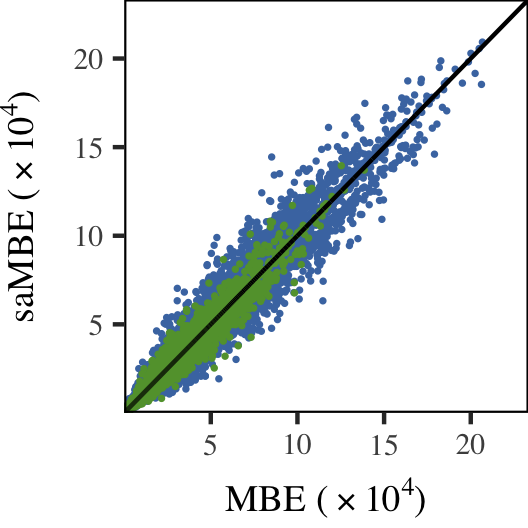
\includegraphics[keepaspectratio=true, width=\textwidth, height=0.23\textheight]{discussion/img/baakman_1_60000_mbe_sambe}
	\caption{dataset \ferdosiOne}
	\label{fig:discussion:singlesphere:mbevssambe:ferdosi1}
\end{subfigure}
% Baakman 1	- MBE
\begin{subfigure}{0.23\textwidth}
	\centering
	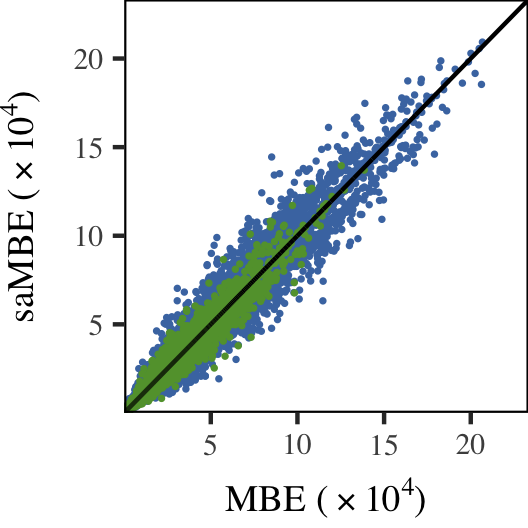
\includegraphics[keepaspectratio=true, width=\textwidth, height=0.23\textheight]{discussion/img/baakman_1_60000_mbe_sambe}
	\caption{dataset \baakmanOne}
	\label{fig:discussion:singlesphere:mbevssambe:baakman1}
\end{subfigure}
% Baakman 4 - MBE
\begin{subfigure}{0.23\textwidth}
	\centering
	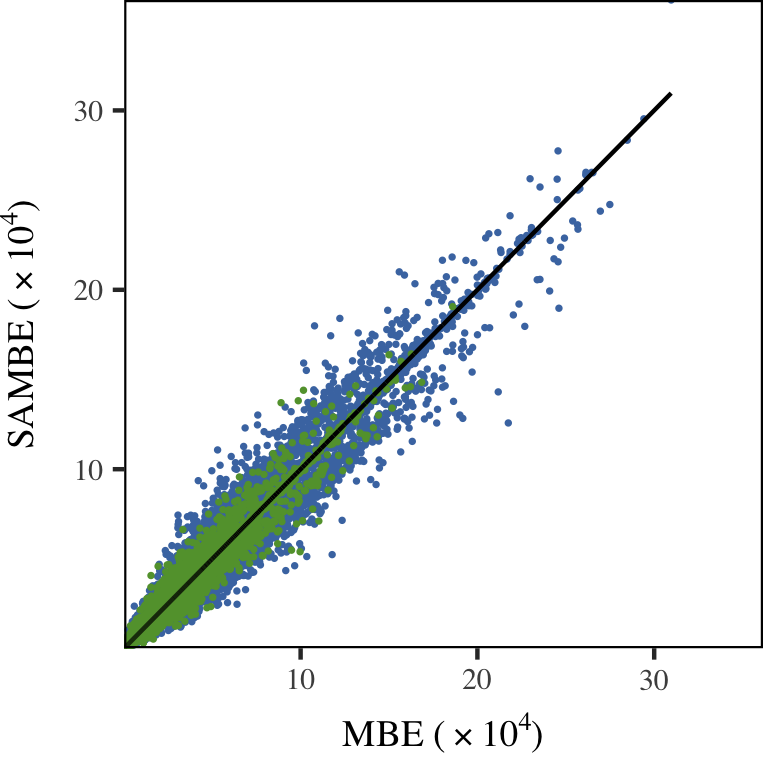
\includegraphics[keepaspectratio=true, width=\textwidth, height=0.23\textheight]{discussion/img/baakman_4_60000_mbe_sambe}
	\caption{dataset \baakmanFour}
	\label{fig:discussion:singlesphere:mbevssambe:baakman4}
\end{subfigure}	
% Baakman 5 - MBE
\begin{subfigure}{0.23\textwidth}
	\centering
	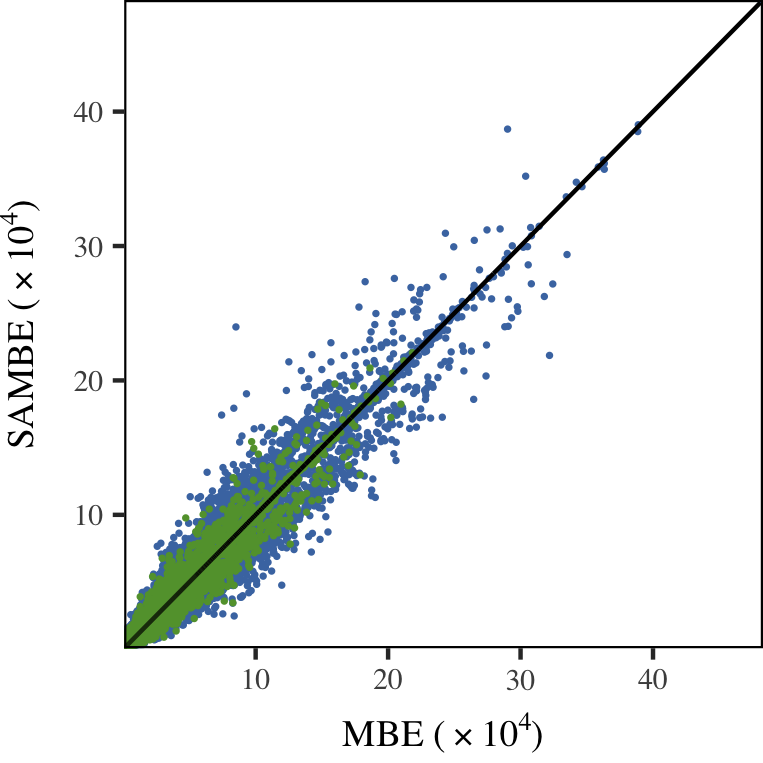
\includegraphics[keepaspectratio=true, width=\textwidth, height=0.23\textheight]{discussion/img/baakman_5_60000_mbe_sambe}
	\caption{dataset \baakmanFive}
	\label{fig:discussion:singlesphere:mbevssambe:baakman5}
\end{subfigure}